\section{Introduction}
\label{sec:intro}
Two generators can have the same global variance while assigning very
different probabilities to parts of the image distribution. For a
few-step sampler, that difference determines what needs to change.
Changing the starting noise can recover image neighborhoods lost during
sampling. A digit that remains absent under several adequate samplers
calls for a test of the training distribution. The two cases require
different controls and different outcomes.

Existing occupancy tests can detect a change in a fixed region
\cite{richardson2018ndb}. To act on that change, however, we need to know
how large it is, what reference it is relative to, and whether an
intervention improves the target without violating fidelity criteria.
An equality test does not answer these questions, and a pooled measure
of spread can stay unchanged while a region is lost.

We therefore fix the reference, the regions, and the effect sizes before
evaluation (Fig.~\ref{fig:pipeline}). A longer teacher sampler measures
the change introduced by a faster sampler, and observed data can reveal an
imbalance shared by both. Conditional spread then measures variation among
samples in the same region or under the same prompt, separately from
regional probability. Each diagnosis motivates one specified change, which
is tested against its control on fresh samples. We ask three questions.
Which regions lose or gain probability relative to a fixed reference?
How does variation within a region or prompt change when fidelity is
measured separately? Which controlled interventions repair the diagnosed
deficit on independent samples?

Two confirmed repairs demonstrate this approach (Fig.~\ref{fig:overview}).
On CIFAR-10, covariance initialization reduces two-call Kernel Inception
Distance (KID) by 32.0\% and increases real-data DINO coverage from 0.206
to 0.288. Evaluating the same outputs against a separate CIFAR-10.1 reference
gives 32.7\% lower KID. On MNIST, signed regional measurements identify
overcorrection after targeted restoration. A separate equal-update
ordinary-data continuation lowers class-mass error by 58.7\% within the
declared fidelity margins.

\begin{figure}[t]
\centering
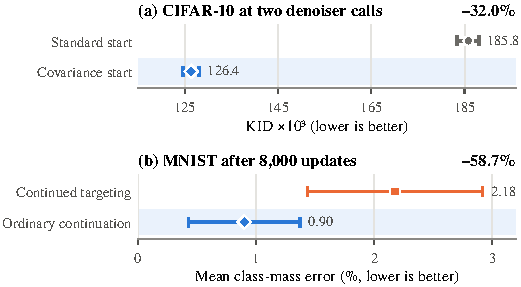
\includegraphics[width=\linewidth]{../figures/overview.pdf}
\caption{Two matched-budget repairs. (a) Covariance start versus standard
start at two denoiser calls on CIFAR-10. (b) Ordinary continuation versus
continued targeting after 8,000 MNIST updates. Bars are 95\% intervals
(Sec.~\ref{sec:metrics}).}
\label{fig:overview}
\end{figure}

A toy example shows why spread alone is not enough. Consider a reference
with probabilities $(1/4,1/2,1/4)$ at feature values $(-2,0,2)$ and a
candidate with equal mass at $-\sqrt{2}$ and $\sqrt{2}$. Both have mean
zero and variance two. The fixed region $[-1/2,1/2]$ contains half the
reference mass and zero candidate mass. If 100 independent draws per
distribution give 50 reference hits and zero candidate hits, the
one-region audit gives a 97.5\% simultaneous upper bound of 0.133 on the
mass ratio. This certifies depletion at the declared threshold of 0.5
(Sec.~\ref{sec:mass}).

Our paper offers the following contributions. First, we introduce a
fixed-reference audit that distinguishes regional loss, within-region
contraction, and departures from reference support, and whose
finite-sample bounds show how the resolution of a regional diagnosis
depends on the effect size, the reference mass, and the comparison family.
Second, we use these diagnoses to design two matched-budget repairs,
a covariance-matched starting noise for a few-step sampler and an
ordinary-data continuation after targeted training, and confirm both on
independent samples. Third, we explain why pooled spread, within-prompt
spread, and comparisons to different teachers can give different answers
about the same generator, using text-to-image models as the test case.

Section~\ref{sec:related} reviews related work, and Sec.~\ref{sec:method}
defines the audit and its guarantees. Section~\ref{sec:experiments}
describes the data, settings, baselines, and metrics.
Section~\ref{sec:results} reports the repairs, the controls, and the
resolution of the audit, and Sec.~\ref{sec:conclusion} concludes.
